% IEEE conference paper
\documentclass[conference]{IEEEtran}
\usepackage{cite}
\usepackage{amsmath,amssymb}
\usepackage{booktabs}
\usepackage{multirow}
\usepackage{array}
\usepackage{graphicx}
\usepackage{xcolor}
\usepackage{url}
\usepackage{tikz}
\usetikzlibrary{arrows.meta,positioning,fit,calc,shapes.geometric,shapes.multipart}
\usepackage{algorithm}
\usepackage{algpseudocode}
\usepackage{balance}
\usepackage[hidelinks]{hyperref}
\graphicspath{{figures/}{diagrams/}}
\newcommand{\system}{the proposed system}
\newcommand{\todo}[1]{\textcolor{red}{#1}}

\title{AI-Based Knowledge Representation and Repository for Enterprise Knowledge Retention}

\author{\IEEEauthorblockN{Atharva}
\IEEEauthorblockA{Independent Researcher\\
Pune, India\\
Author contact withheld for artifact preparation}}

\begin{document}
\maketitle

\begin{abstract}
Enterprise knowledge is distributed across documents, meeting records, spreadsheets, images, audio, and collaboration systems. Keyword search recovers lexical matches but does not preserve why a decision was made, who participated, what alternatives were rejected, or what downstream impact may follow. Retrieval-augmented generation improves access to unstructured evidence, yet text-only retrieval is weak when the answer depends on relationships among people, decisions, reasons, and projects. This paper presents \system, an implemented organizational-memory platform that combines multi-source ingestion, structured decision extraction, a Neo4j property graph, Chroma vector retrieval, and LangGraph/LangChain agents. A router classifies a question as historical query or impact analysis; specialized agents invoke graph and raw-memory tools under project and source constraints, and the response includes a trace of the evidence-retrieval actions. The system supports PDF, image, spreadsheet, and audio inputs, with Slack and Microsoft Teams integration points, FastAPI services, a Next.js interface, Supabase application services, and selectable Groq or local Ollama language-model providers. We formalize the graph, vector, and hybrid retrieval objectives and specify an evaluation protocol covering retrieval, answer faithfulness, source attribution, latency, and resource use. Because the repository does not contain a controlled benchmark or measured experiment log, this paper reports implementation evidence and reproducible evaluation procedures rather than invented numerical results. The contribution is a modular, source-grounded architecture for decision memory and impact-oriented question answering, together with explicit safeguards for scope filtering, provenance, and deployment limitations.
\end{abstract}

\begin{IEEEkeywords}
organizational memory, knowledge graph, GraphRAG, retrieval-augmented generation, multi-agent systems, decision intelligence, source attribution, enterprise search
\end{IEEEkeywords}

\section{Introduction}
Organizations accumulate knowledge faster than they can curate it. A decision may first appear in a meeting, be justified in a PDF, refined in a spreadsheet, discussed in a chat channel, and operationalized by a different team. The resulting evidence is fragmented across incompatible representations and access boundaries. When an employee changes role or leaves the organization, the information may remain technically stored but become practically inaccessible: the organization has retained artifacts but lost the decision context that connects them.

Traditional enterprise search addresses only part of this problem. Lexical retrieval is effective when a user knows the exact terminology used in the source, but it is brittle under paraphrase and cannot directly answer relational questions such as who approved a migration, which alternatives were considered, or what other decisions depend on a component. Neural retrieval improves semantic matching but still tends to return independent passages. A conventional retrieval-augmented generation (RAG) pipeline then asks a language model to reconstruct relationships from a small set of text chunks. That reconstruction can be useful, but it is difficult to audit and may omit the edges that make an organizational explanation meaningful.

Knowledge graphs provide a complementary representation. A decision can be connected to its topic, reasons, alternatives, people, source, project, and timestamp. Graph traversal makes those relationships explicit, while vector search retains the unstructured evidence needed to preserve nuance. Recent GraphRAG studies show that graph construction, indexing, retrieval, and generation are separate design choices rather than a single algorithm \cite{zhou2025graph,han2025graphrag,cao2024lego}. Enterprise use-case research likewise emphasizes that knowledge-graph construction and maintenance must be considered together with the downstream question-answering task \cite{schneider2024enterprise,barros2024empwr}. Multi-agent KGQA work further motivates separating routing, entity and relationship retrieval, and answer synthesis \cite{nguyen2025scigent}.

This paper presents \system, a working software system whose central abstraction is organizational decision memory. The implementation ingests several source types, extracts structured knowledge using schema-constrained language-model calls, persists decision projections in Neo4j, indexes raw text in Chroma, and exposes source-grounded query and impact-analysis agents through a FastAPI service and Next.js client. The system is designed around a conservative answer policy: agents must answer from tool results, respect an exact source filter when present, and return source traces. The architecture therefore treats provenance as a first-class output rather than a post-processing annotation.

The paper makes the following contributions:
\begin{enumerate}
\item A decision-centric organizational-memory architecture that combines property-graph structure with raw-memory vector retrieval.
\item A multi-agent query design that separates historical questions from ``what-if'' impact questions and provides distinct tool affordances.
\item A multi-source ingestion pipeline covering PDFs, images, spreadsheets, audio, meeting text, and collaboration-system integration points.
\item A source- and project-scoped retrieval policy that constrains both tool arguments and final answer synthesis.
\item Formal definitions for graph retrieval, vector retrieval, score fusion, confidence, and source-trace completeness.
\item A reproducible evaluation protocol that distinguishes implemented behavior from results that require a controlled dataset and measurement run.
\end{enumerate}

\section{Background and Related Work}
\subsection{RAG and GraphRAG}
RAG combines a parametric generator with a non-parametric store \cite{lewis2020rag}. Dense retrieval is robust to vocabulary variation, but chunk-level retrieval does not inherently encode multi-hop dependencies. GraphRAG augments the retrieval unit with nodes, edges, communities, or subgraphs. Surveys classify systems by graph type, indexed components, retrieval primitive, and retrieval granularity \cite{han2025graphrag}. The recent unified analysis by Zhou \emph{et al.} demonstrates that graph construction, index construction, operator configuration, and retrieval/generation must be evaluated separately \cite{zhou2025graph}. \system adopts a deliberately lightweight property graph rather than a community-detection pipeline: the graph is centered on decisions and their evidence-bearing relations, while Chroma preserves text chunks for semantic recall.

\subsection{Knowledge-graph question answering}
Knowledge-graph question answering traditionally maps natural-language questions to structured queries, including SPARQL or Cypher. The difficulty is not only query generation but entity and relation resolution under open-ended user language. SCIGENT addresses this by separating end-to-end question answering into cooperating agents and evaluates entity, query, and end-to-end behavior \cite{nguyen2025scigent}. \system shares the separation principle but uses bounded LangChain tools over application-owned Neo4j and Chroma stores. This avoids exposing arbitrary database-query generation to the user-facing agent and makes the evidence path inspectable.

\subsection{Enterprise knowledge management and decision support}
Enterprise KG research identifies knowledge acquisition, maintenance, reasoning, and governance as coupled concerns \cite{schneider2024enterprise,barros2024empwr}. Industrial risk-analysis work shows how graph-enhanced RAG can connect structured failure information to textual evidence and improve reasoning over effects and causes \cite{bahr2025fmea}. These observations motivate a decision-centric schema in which a reason, alternative, impact, and responsible person are stored as explicit neighbors rather than left only inside a passage.

\subsection{Temporal and provenance concerns}
Knowledge in organizations changes. A decision may be superseded, and a source may represent a plan rather than an executed action. Temporal GraphRAG research identifies temporal ambiguity and redundancy as causes of retrieval failure \cite{li2025tgrag}. The present implementation stores an optional timestamp and source on decision nodes but does not yet implement temporal validity intervals or conflict resolution. We therefore treat temporal GraphRAG, version-aware edges, and conflict detection as future work rather than claiming capabilities not present in the repository.

\begin{table}[t]
\caption{Positioning of organizational-memory approaches.}
\label{tab:comparison}
\centering\small
\begin{tabular}{p{1.35cm}p{1.2cm}p{1.3cm}p{1.35cm}p{1.3cm}}
\toprule
Approach & Semantic retrieval & Relationship reasoning & Traceability & Main limitation\\
\midrule
Keyword search & Low & No & Source link & Vocabulary and silo dependence\\
Vanilla RAG & High & Implicit & Passage context & Relations reconstructed by generator\\
GraphRAG & High & Explicit & Graph evidence & Graph construction and freshness\\
\system & High & Decision-centered & Tool/source trace & No temporal conflict model yet\\
\bottomrule
\end{tabular}
\end{table}

\section{Problem Formulation}
Let an organization contain a set of sources $S$, documents and transcripts $D$, and a decision graph $G=(V,E)$. A decision record is represented by the tuple
\begin{equation}
 d=(a,t,r,i,A,P,\tau,s,p),
\end{equation}
where $a$ is the action, $t$ the topic, $r$ the reason, $i$ the impact, $A$ alternatives, $P$ people, $\tau$ an optional timestamp, $s$ the source, and $p$ the project. The system must answer two classes of question: historical query $q_h$ (what, why, who, when) and impact query $q_i$ (what changes, breaks, or is affected if a decision changes).

The design objective is not to maximize a single language-model score. It is to return an answer $y$ that is relevant to $q$, supported by retrieved evidence $R(q)$, scoped to the requested source/project, and accompanied by a trace $T(q)$. We write:
\begin{equation}
 y = \operatorname{Gen}(q, R_g(q), R_v(q), T(q)),
\end{equation}
where $R_g$ is structured graph evidence and $R_v$ is raw-memory evidence. A valid answer satisfies $\operatorname{scope}(R,q)=1$ and $\operatorname{support}(y,R)=1$ under the system's answer policy. These predicates are evaluated by human or automated annotation in the proposed benchmark; they are not assumed to be guaranteed by the language model.

\section{System Architecture}
Figure~\ref{fig:architecture} shows the implemented logical architecture. The browser client is a Next.js/React application with authentication, project, graph, query, activity, file, and team views. FastAPI routes mediate upload, query, graph, project, activity, health, and collaboration operations. Application services isolate persistence and authorization concerns from ingestion and agent orchestration.

\begin{figure*}[t]
\centering
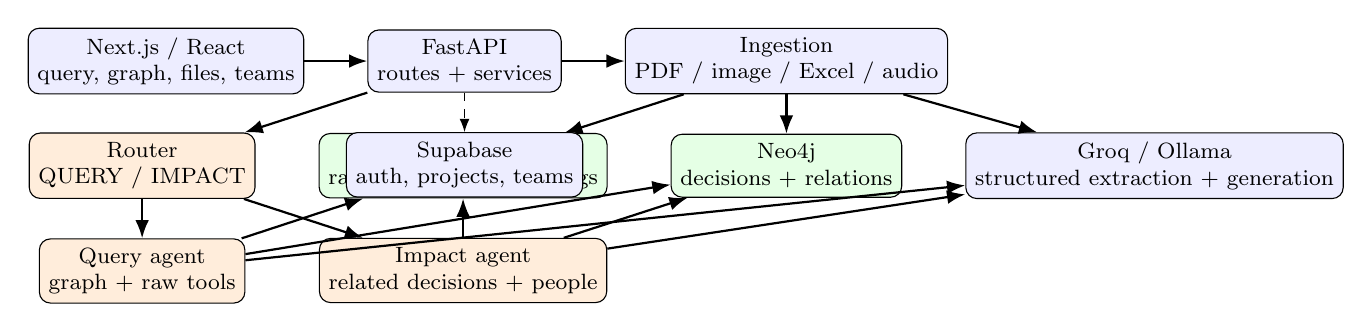
\begin{tikzpicture}[font=\footnotesize,>=Latex,node distance=5mm and 8mm,
 box/.style={draw,rounded corners,align=center,minimum height=7mm,minimum width=21mm,fill=blue!7},
 store/.style={draw,rounded corners,align=center,minimum height=8mm,minimum width=24mm,fill=green!10},
 agent/.style={draw,rounded corners,align=center,minimum height=8mm,minimum width=25mm,fill=orange!14},
 line/.style={->,thick}]
\node[box] (ui) {Next.js / React\\query, graph, files, teams};
\node[box,right=of ui] (api) {FastAPI\\routes + services};
\node[box,right=of api] (ing) {Ingestion\\PDF / image / Excel / audio};
\node[store,below=of ing] (neo) {Neo4j\\decisions + relations};
\node[store,left=of neo] (chroma) {Chroma\\raw chunks + embeddings};
\node[agent,left=of chroma] (router) {Router\\QUERY / IMPACT};
\node[agent,below=of router] (q) {Query agent\\graph + raw tools};
\node[agent,below=of chroma] (i) {Impact agent\\related decisions + people};
\node[box,right=of neo] (llm) {Groq / Ollama\\structured extraction + generation};
\node[box,below=of api] (auth) {Supabase\\auth, projects, teams};
\draw[line] (ui)--(api);
\draw[line] (api)--(ing);
\draw[line] (api)--(router);
\draw[line] (ing)--(neo);
\draw[line] (ing)--(chroma);
\draw[line] (router)--(q);
\draw[line] (router)--(i);
\draw[line] (q)--(neo);
\draw[line] (q)--(chroma);
\draw[line] (i)--(neo);
\draw[line] (i)--(chroma);
\draw[line] (ing)--(llm);
\draw[line] (q)--(llm);
\draw[line] (i)--(llm);
\draw[dashed,->] (api)--(auth);
\end{tikzpicture}

\caption{Logical architecture of \system. Solid arrows are implemented data paths; dashed arrows denote integration or provider selection points.}
\label{fig:architecture}
\end{figure*}

The ingestion path detects the file extension and dispatches to PyMuPDF for PDF text, OpenPyXL-based extraction for spreadsheets, image extraction for raster inputs, and audio transcription for supported audio/video formats. Meeting text has a dedicated extraction schema with categories such as decision, action item, risk, requirement, participant, deadline, and technology. Generic content is chunked, passed through schema-constrained extraction, and projected into Neo4j; raw content is stored as embeddings in Chroma when the vector path is enabled.

The query path first routes the question to QUERY or IMPACT. The query agent uses structured decision search and raw-memory search. The impact agent uses related-decision search, person-based search, and raw-memory search. Both agents enforce optional $source\_filter$ and $project\_id$ parameters and return an answer, a textual reasoning summary of tools used, and a source trace containing tool names, arguments, and result previews.

\subsection{Knowledge graph model}
The core graph uses Organization and Project containers; Decision nodes connect to Person through MADE\_BY, Reason through BASED\_ON, Alternative through ALTERNATIVE, and Project through BELONGS\_TO. Meeting ingestion adds Meeting and MeetingKnowledge nodes, with HAS\_KNOWLEDGE and INVOLVES relations. Source, impact, timestamp, project, and organization are properties on decision or knowledge nodes. Figure~\ref{fig:schema} abstracts the model without implying node types not present in the code.

\begin{figure}[t]
\centering
\resizebox{\columnwidth}{!}{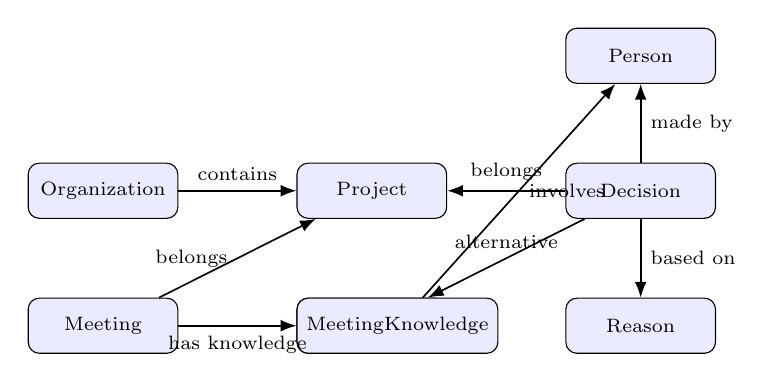
\begin{tikzpicture}[font=\scriptsize,>=Latex,node distance=10mm and 15mm,
 n/.style={draw,rounded corners,align=center,minimum width=19mm,minimum height=7mm,fill=blue!8},
 r/.style={draw,ellipse,align=center,inner sep=1.5pt,fill=orange!12},
 e/.style={->,semithick}]
\node[n] (org) {Organization};
\node[n,right=of org] (proj) {Project};
\node[n,right=of proj] (dec) {Decision};
\node[n,above=of dec] (person) {Person};
\node[n,below=of dec] (reason) {Reason};
\node[n,below=of proj] (alt) {Alternative};
\node[n,below=of org] (meet) {Meeting};
\node[n,right=of meet] (mk) {MeetingKnowledge};
\draw[e] (org)--(proj) node[midway,above]{contains};
\draw[e] (dec)--(proj) node[midway,above]{belongs};
\draw[e] (dec)--(person) node[midway,right]{made by};
\draw[e] (dec)--(reason) node[midway,right]{based on};
\draw[e] (dec)--(alt) node[midway,above]{alternative};
\draw[e] (meet)--(proj) node[midway,left]{belongs};
\draw[e] (meet)--(mk) node[midway,below]{has knowledge};
\draw[e] (mk)--(person) node[midway,right]{involves};
\end{tikzpicture}
}
\caption{Decision-centric knowledge-graph schema.}
\label{fig:schema}
\end{figure}

\subsection{Vector memory and hybrid retrieval}
Chroma stores overlapping text chunks with source and optional project metadata. Each chunk is embedded using the configured Cohere embedding model. At query time, the vector tool computes a query embedding and requests the nearest chunks, then performs a second hard-filter check so a result with an incorrect source or project is discarded. Neo4j search uses case-insensitive word containment over decision, subject, reason, and person fields. The system therefore combines high-precision structured retrieval with semantically broad raw-memory retrieval, but the current implementation does not expose a learned fusion weight or a benchmark-calibrated ranker.

\subsection{Model providers and application boundary}
Groq is the default cloud model provider with Llama 3.3 70B Versatile; Ollama can be selected for local execution and falls back to Groq if unreachable. Supabase services support application-level authentication and project/team workflows. The provider factory is intentionally isolated from agents so a deployment can change model locality without changing graph or vector tools. This separation is useful for privacy analysis, although it does not by itself guarantee that no sensitive data leaves the deployment.

\section{Ingestion and Knowledge Construction}
\subsection{Multimodal ingestion}
The input dispatcher accepts PDF, XLS/XLSX, PNG/JPG/GIF/WEBP, and common audio/video extensions. PDF extraction uses page text from PyMuPDF. Spreadsheet extraction is delegated to an Excel utility. Image extraction and audio transcription are separate services, allowing deployments to replace the provider or add OCR/transcription controls. Slack ingestion and Microsoft Teams integration are represented by dedicated modules; their operational completeness depends on credentials and upstream API availability.

\subsection{Structured extraction}
Generic extraction returns a list of decision items with fields decision, reason, impact, alternatives, people, timestamp, and topic. A Pydantic schema is passed to the model through structured output. Long input is split by paragraphs with a provider-dependent maximum chunk length; each successful chunk result contributes only items with non-empty decisions. Meeting extraction uses a richer schema and stores the raw meeting text in Chroma before persisting structured items.

\begin{algorithm}[t]
\caption{Document ingestion and graph projection}
\label{alg:ingest}
\begin{algorithmic}[1]
\Require bytes $b$, filename $f$, source $s$, provider $m$
\State $x\gets\operatorname{Decode}(b,\operatorname{suffix}(f))$
\State $C\gets\operatorname{Chunk}(x)$
\State $I\gets\emptyset$
\ForAll{$c\in C$}
  \State $I\gets I\cup\operatorname{ExtractDecision}(c,m)$
\EndFor
\ForAll{$d\in I$}
  \State $\operatorname{Neo4jCreate}(d,s,project,organization)$
\EndFor
\State $\operatorname{ChromaAdd}(\operatorname{OverlapChunks}(x),s,project)$
\State \Return $I$
\end{algorithmic}
\end{algorithm}

\subsection{Graph construction and evidence preservation}
Neo4j persistence uses MERGE for organization, project, person, alternative, and reason nodes, while each extracted decision receives a unique identifier. The raw source is retained separately in Chroma so that a structured record can be checked against the underlying text. The two projections are not transactionally coupled in the legacy ingestion path; application services can disable the projections and commit an authoritative transaction before writing them. This is an important boundary for deployment: a successful graph write does not prove that every vector write succeeded, and a vector duplicate is treated as a no-op by the Chroma adapter.

\section{Multi-Agent Query Processing}
The router prompts the selected LLM to emit one of two labels. IMPACT is selected when the question asks what would happen, what breaks, what changes, or what risks arise. All other questions are routed to QUERY. This coarse classification is intentionally simple and transparent; it is not a learned intent model and can misclassify ambiguous questions.

The QUERY agent prioritizes $search\_decisions$ and uses $search\_raw\_memory$ for additional context or when structured search returns nothing. The IMPACT agent searches related decisions, optionally searches by person, and retrieves raw context. Both use a bounded tool loop; local Ollama mode uses direct tool execution and feeds the resulting context to the base model. Tool-call errors can trigger a direct-execution fallback. The final prompt prohibits general knowledge, raw transcript dumping, and mixing sources under an active filter.

\begin{figure}[t]
\centering
\resizebox{\columnwidth}{!}{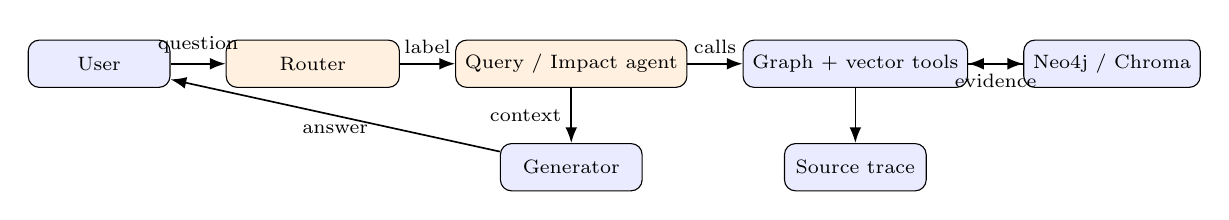
\begin{tikzpicture}[font=\scriptsize,>=Latex,node distance=7mm,
 s/.style={draw,rounded corners,align=center,minimum width=18mm,minimum height=6mm,fill=blue!8},
 a/.style={draw,rounded corners,align=center,minimum width=22mm,minimum height=6mm,fill=orange!12},
 d/.style={->,semithick}]
\node[s] (u) {User};
\node[a,right=of u] (r) {Router};
\node[a,right=of r] (ag) {Query / Impact agent};
\node[s,right=of ag] (t) {Graph + vector tools};
\node[s,right=of t] (db) {Neo4j / Chroma};
\node[s,below=of ag] (g) {Generator};
\node[s,below=of t] (tr) {Source trace};
\draw[d] (u)--(r) node[midway,above]{question};
\draw[d] (r)--(ag) node[midway,above]{label};
\draw[d] (ag)--(t) node[midway,above]{calls};
\draw[d] (t)--(db);
\draw[d] (db)--(t) node[midway,below]{evidence};
\draw[d] (ag)--(g) node[midway,left]{context};
\draw[d] (t)--(tr);
\draw[d] (g)--(u) node[midway,below]{answer};
\end{tikzpicture}
}
\caption{Query routing, retrieval, reasoning, and source-trace emission.}
\label{fig:agent}
\end{figure}

\begin{algorithm}[t]
\caption{Scoped hybrid query}
\label{alg:query}
\begin{algorithmic}[1]
\Require question $q$, optional source $s$, project $p$
\State $k\gets\operatorname{Route}(q)$
\If{$k=\textsc{Query}$}
  \State $G\gets\operatorname{NeoSearch}(q,s,p)$
\Else
  \State $G\gets\operatorname{ImpactSearch}(q,s,p)$
\EndIf
\State $V\gets\operatorname{VectorSearch}(q,s,p)$
\State $R\gets\operatorname{Filter}(G\cup V,s,p)$
\State $y\gets\operatorname{Generate}(q,R,\operatorname{Trace}(G,V))$
\State \Return $(y,R,\operatorname{Trace})$
\end{algorithmic}
\end{algorithm}

\section{Formal Retrieval and Attribution Model}
Let a text chunk embedding be $\mathbf{e}_d\in\mathbb{R}^n$ and the query embedding be $\mathbf{e}_q$. Cosine similarity is
\begin{equation}
 \operatorname{cos}(q,d)=\frac{\mathbf{e}_q\cdot\mathbf{e}_d}{\|\mathbf{e}_q\|_2\|\mathbf{e}_d\|_2}.
\end{equation}
For a graph candidate $v$, define a normalized graph score
\begin{equation}
 g(q,v)=w_t\operatorname{match}(q,topic_v)+w_a\operatorname{match}(q,action_v)+w_r\operatorname{match}(q,reason_v)+w_p\operatorname{match}(q,people_v),
\end{equation}
where the weights are an evaluation parameter, not a value hard-coded by the current implementation. A general hybrid ranker can be expressed as
\begin{equation}
 H(q,z)=\lambda\,\widetilde{g}(q,z)+(1-\lambda)\,\widetilde{v}(q,z),\quad 0\leq\lambda\leq1,
\end{equation}
with min--max or reciprocal-rank normalization. In the current system, graph and vector tools are invoked as separate evidence channels and the LLM receives their results; $H$ is therefore a design formalization for controlled evaluation rather than a claim about a learned production ranker.

For a path $\pi=(v_0,r_1,v_1,\ldots,v_l)$, a traversal score may be defined as
\begin{equation}
 T(\pi|q)=\sum_{j=0}^{l}\gamma^j g(q,v_j)+\sum_{j=1}^{l}\eta(r_j),
\end{equation}
where $\gamma$ discounts distance and $\eta$ encodes relation relevance. An answer confidence estimate can combine evidence coverage, source agreement, and scope compliance:
\begin{equation}
 C(y|q)=\alpha\,cov(y,R)+\beta\,agr(R)+\delta\,scope(R,q),\quad \alpha+\beta+\delta=1.
\end{equation}
The implementation exposes source traces but does not yet calculate $C$ automatically; this equation defines a measurable future evaluation target.

\section{Implementation}
Table~\ref{tab:stack} summarizes the observed technology stack. The frontend is Next.js with React, TypeScript, Tailwind-based styling, Framer Motion/GSAP components, and Supabase client integration. The backend is Python/FastAPI with Pydantic settings, JWT-related security modules, application services, route modules, and logging configuration. LangChain supplies message, prompt, tool, and structured-output abstractions; LangGraph is used for agent orchestration in the broader application design. Neo4j provides graph persistence, while Chroma and Cohere provide vector storage and embeddings. PyMuPDF, OpenPyXL, audio transcription, image extraction, Slack SDK, and Microsoft Teams integration cover the ingestion boundary.

\begin{table}[t]
\caption{Implemented technology stack evidenced by the repository.}
\label{tab:stack}
\centering\small
\begin{tabular}{p{1.7cm}p{4.7cm}}
\toprule
Layer & Components\\
\midrule
Client & Next.js, React, TypeScript, Tailwind, Framer Motion, GSAP\\
API & FastAPI, Uvicorn, Pydantic settings, multipart uploads\\
Agents & LangChain, LangGraph, Groq Llama 3.3, Ollama fallback\\
Structured store & Neo4j property graph, Cypher\\
Vector store & Chroma Cloud/client, Cohere embeddings\\
Ingestion & PyMuPDF, OpenPyXL, image extraction, audio transcription\\
Application & Supabase, JWT utilities, projects, teams, activity\\
Integrations & Slack SDK and Microsoft Teams service boundary\\
\bottomrule
\end{tabular}
\end{table}

Security is implemented at the application boundary through authentication services, token handling, organization/project identifiers, and source/project filters. Nevertheless, access control should be independently audited before production deployment. In particular, a prompt instruction is not a substitute for a database authorization rule; every storage query should be tested against cross-project and cross-organization cases.

\section{Evaluation Protocol}
\subsection{Evaluation status and reproducibility}
The repository contains unit and integration test modules, but it does not provide a frozen corpus, ground-truth annotations, controlled hardware log, or completed benchmark results. Accordingly, the tables in this section specify what should be measured and how; they do not fabricate values. A publication-ready empirical extension should release the corpus manifest, question set, gold evidence, model/provider versions, timestamps, and raw traces.

\subsection{Dataset and question design}
Build a de-identified organizational corpus from representative PDFs, meeting transcripts, spreadsheets, images, and audio. Partition by source and by project to prevent leakage. Annotate each question with answer type (what, why, who, when, impact), gold source set, gold decision nodes, expected people/reasons/alternatives, and whether multi-hop traversal is required. Include adversarial questions whose terminology differs from the source and scope tests that request a single source. A database-migration scenario is suitable as a case study only when its source artifacts and labels are actually available.

\subsection{Metrics}
Retrieval precision, recall, and F1 are computed over gold evidence items. Retrieval accuracy measures whether at least one gold decision or supporting chunk is returned in the top-$k$. Answer faithfulness is judged against evidence, while source-attribution accuracy checks whether every cited source is in the gold or retrieved support set. Impact quality should be scored by coverage of affected decisions and people, unsupported-claim rate, and risk-label agreement. System metrics include end-to-end response time, graph-query time, embedding-search time, tool-loop count, memory usage, and ingestion throughput.

\begin{table}[t]
\caption{Evaluation matrix to be populated by a controlled run.}
\label{tab:eval}
\centering\scriptsize
\begin{tabular}{p{1.45cm}p{2.15cm}p{2.55cm}}
\toprule
Metric & Unit & Required evidence\\
\midrule
P/R/F1 & fraction & gold nodes/chunks and top-$k$ traces\\
Retrieval accuracy & fraction & question-level hit labels\\
Faithfulness & rubric score & answer--evidence annotations\\
Attribution accuracy & fraction & cited source vs. gold source\\
Graph latency & ms & Neo4j query timestamps\\
Vector latency & ms & embedding and Chroma timestamps\\
Response time & ms & request start/end logs\\
Memory use & MB & process/container telemetry\\
Impact coverage & fraction & affected-node annotation\\
\bottomrule
\end{tabular}
\end{table}

Baselines should include keyword search, vector-only RAG, graph-only retrieval, and the full two-agent system. Ablations should remove source filtering, remove graph retrieval, remove raw-memory retrieval, replace the router with a single agent, and compare Groq with Ollama when the same model family and prompt are available. Statistical reporting should include per-question scores, confidence intervals, and failure categories; a single average score is insufficient for an enterprise-memory system.

\section{Case Study: Decision-Migration Reasoning}
The intended case-study pattern is a database migration. A source artifact describes a decision to move from one database to another, records scaling or reliability reasons, names participants, and lists alternatives. Ingestion produces a Decision node connected to Reason, Alternative, Person, Project, and Source properties; raw chunks remain in Chroma. A historical question such as ``Why did the team migrate?'' routes to QUERY, which prioritizes the structured decision and retrieves raw context if necessary. An impact question such as ``What would be affected if the migration were reversed?'' routes to IMPACT and searches related decisions and people before synthesizing an assessment.

This case illustrates the intended reasoning path, not a measured result. The answer is valid only if the migration artifact is present in the deployed corpus and the returned evidence supports the claim. If a source filter is active and the artifact is absent, the agent is instructed to return no information for that source rather than merge evidence from other files.

\section{Discussion}
The main strength of \system is the alignment between the representation and the question types. Decisions, reasons, alternatives, people, and impacts are individually addressable, while raw text retains details that are difficult to normalize. The router also creates an operational distinction between historical recall and impact exploration. Finally, traces expose the tools and scope arguments used to produce an answer, which supports debugging and human review.

The design has several weaknesses. Extraction quality depends on the selected LLM and the quality of source text. OCR and transcription errors can enter both projections. The current graph search is primarily property matching rather than a learned semantic graph retriever, and the vector and graph channels are not fused by a calibrated score. Agent prompts reduce unsupported generation but cannot provide formal guarantees. Ingestion can depend on external APIs for language models, embeddings, Slack, Teams, and hosted databases. Synchronous work and retries may become expensive for large files or high request concurrency.

Privacy requires particular care because organizational memory may include sensitive personnel, customer, or security information. Local Ollama execution can reduce data egress for generation, but embedding providers and hosted databases remain separate privacy surfaces. A production deployment should add tenant-isolated database constraints, role-based access control, encrypted secrets, retention policies, deletion verification across both stores, and audit logs that distinguish user-visible provenance from sensitive internal trace data.

\section{Limitations and Future Work}
The implementation does not yet provide temporal validity intervals, version-aware graph updates, automated knowledge-conflict detection, a learned hybrid ranker, a released benchmark, or measured end-to-end results. Meeting and collaboration integrations are present as code boundaries but require operational credentials and source-specific synchronization logic. Large-scale deployments will need asynchronous ingestion, queueing, back-pressure, idempotent job identifiers, and observability for external provider failures.

Future work should extend the schema with valid-from/valid-to intervals and supersession edges, then evaluate temporal GraphRAG methods against organizational questions. Incremental updates should reconcile changed documents instead of appending duplicate projections. Multi-tenancy and RBAC should be enforced in Neo4j and Chroma query predicates rather than only in prompts. Additional connectors could cover Microsoft Teams, Google Drive, SharePoint, Jira, and email. A public or synthetic benchmark should include decision chains, provenance labels, scope violations, temporal conflicts, and impact questions. Finally, calibrated confidence, human feedback, and conflict-aware explanations could make the system safer for operational decision support.

\section{Conclusion}
This paper presented \system, an implemented multi-agent organizational-memory platform that joins source ingestion, structured decision graphs, vector memory, scoped retrieval, and source-traceable answer generation. Its central design choice is to represent organizational decisions and their reasons, alternatives, people, and impacts explicitly while preserving the source text needed for verification. A QUERY agent supports historical recall, an IMPACT agent supports downstream reasoning, and both are constrained by project and source filters. The repository supports a credible prototype architecture, but it does not contain the controlled benchmark needed to claim numerical improvements. The evaluation protocol therefore makes the next empirical step explicit: release a corpus and gold evidence, compare graph and vector baselines, measure attribution and latency, and report failure modes. With temporal modeling, stronger authorization, asynchronous ingestion, and calibrated evaluation, decision-centric GraphRAG can become a practical foundation for preserving organizational memory without obscuring the provenance on which enterprise trust depends.

\balance
\nocite{*}
\bibliographystyle{IEEEtran}
\bibliography{references}
\end{document}
